\documentclass[a4paper]{article}
\usepackage{vntex}
\usepackage{a4wide,amssymb,epsfig,latexsym,multicol,array,hhline,fancyhdr}
\usepackage{booktabs}
\usepackage{amsmath}
\usepackage{lastpage}
\usepackage[lined,boxed,commentsnumbered]{algorithm2e}
\usepackage{enumerate}
\usepackage{color}
\usepackage{graphicx}							% Standard graphics package
\usepackage{array}
\usepackage{tabularx, caption}
\usepackage{multirow}
\usepackage[framemethod=tikz]{mdframed}% For highlighting paragraph backgrounds
\usepackage{multicol}
\usepackage{rotating}
\usepackage{graphics}
\usepackage{geometry}
\usepackage{setspace}
\usepackage{epsfig}
\usepackage{tikz}
\usepackage{listings}
\usetikzlibrary{arrows,snakes,backgrounds}
\usepackage{hyperref}
\hypersetup{urlcolor=blue,linkcolor=black,citecolor=black,colorlinks=true} 
%\usepackage{pstcol} 								% PSTricks with the standard color package

\newtheorem{theorem}{{\bf Định lý}}
\newtheorem{property}{{\bf Tính chất}}
\newtheorem{proposition}{{\bf Mệnh đề}}
\newtheorem{corollary}[proposition]{{\bf Hệ quả}}
\newtheorem{lemma}[proposition]{{\bf Bổ đề}}

\everymath{\color{blue}}
%\usepackage{fancyhdr}
\setlength{\headheight}{40pt}
\pagestyle{fancy}
\fancyhead{} % clear all header fields
\fancyhead[L]{
 \begin{tabular}{rl}
    \begin{picture}(25,15)(0,0)
    \put(0,-8){
\includegraphics[width=8mm, height=8mm]{logoITSGUsmall.png}}
    %\put(0,-8){\epsfig{width=10mm,figure=hcmut.eps}}
   \end{picture}&
	%\includegraphics[width=8mm, height=8mm]{hcmut.png} & %
	\begin{tabular}{l}
		\textbf{\bf \ttfamily Trường Đại học Sài Gòn}\\
		\textbf{\bf \ttfamily Khoa Công Nghệ Thông Tin}
	\end{tabular} 	
 \end{tabular}
}
\fancyhead[R]{
	\begin{tabular}{l}
		\tiny \bf \\
		\tiny \bf 
	\end{tabular}  }
\fancyfoot{} % clear all footer fields
\fancyfoot[L]{\scriptsize \ttfamily Bài tập lớn môn Phát triển phần mềm mã nguồn mở - Niên khóa 2023-2024}
\fancyfoot[R]{\scriptsize \ttfamily Trang {\thepage}/\pageref{LastPage}}
\renewcommand{\headrulewidth}{0.3pt}
\renewcommand{\footrulewidth}{0.3pt}


%%%
\setcounter{secnumdepth}{4}
\setcounter{tocdepth}{3}
\makeatletter
\newcounter {subsubsubsection}[subsubsection]
\renewcommand\thesubsubsubsection{\thesubsubsection .\@alph\c@subsubsubsection}
\newcommand\subsubsubsection{\@startsection{subsubsubsection}{4}{\z@}%
                                     {-3.25ex\@plus -1ex \@minus -.2ex}%
                                     {1.5ex \@plus .2ex}%
                                     {\normalfont\normalsize\bfseries}}
\newcommand*\l@subsubsubsection{\@dottedtocline{3}{10.0em}{4.1em}}
\newcommand*{\subsubsubsectionmark}[1]{}
\makeatother

\definecolor{dkgreen}{rgb}{0,0.6,0}
\definecolor{gray}{rgb}{0.5,0.5,0.5}
\definecolor{mauve}{rgb}{0.58,0,0.82}

\lstset{frame=tb,
	language=Matlab,
	aboveskip=3mm,
	belowskip=3mm,
	showstringspaces=false,
	columns=flexible,
	basicstyle={\small\ttfamily},
	numbers=none,
	numberstyle=\tiny\color{gray},
	keywordstyle=\color{blue},
	commentstyle=\color{dkgreen},
	stringstyle=\color{mauve},
	breaklines=true,
	breakatwhitespace=true,
	tabsize=3,
	numbers=left,
	stepnumber=1,
	numbersep=1pt,    
	firstnumber=1,
	numberfirstline=true
}

\begin{document}

\begin{titlepage}
	\begin{center}
		TRƯỜNG ĐẠI HỌC SÀI GÒN \\
		KHOA CÔNG NGHỆ THÔNG TIN
	\end{center}
	\vspace{1cm}

	\begin{figure}[h!]
		\begin{center}
			
\includegraphics[width=3cm]{logoITSGU.png}
		\end{center}
	\end{figure}

	\vspace{1cm}


	\begin{center}
		\begin{tabular}{c}
			\multicolumn{1}{l}{\textbf{{\Large PHÁT TRIỂN PHẦN MỀM MÃ NGUỒN MỞ}}} \\
			~~                                                                    \\
			\hline
			\\
			\multicolumn{1}{l}{\textbf{{\Large Phát triển}}}                      \\
			\\

			\textbf{{\Huge Ứng dụng nghe nhạc trên PYTHON}}                       \\
			\\
			\hline
		\end{tabular}
	\end{center}

	\vspace{3cm}

	\begin{table}[h]
		\begin{tabular}{rrl}
			\hspace{5 cm} & GVHD: & Từ Lãng Phiêu                     \\
			              & SV:   & Nguyễn Anh Danh - 3121410103      \\
			              &       & Phan Duy - 3121410003             \\
			              &       & Văn Phú Hiếu - 3121410201         \\
			              &       & Đỗ Nguyễn Hoàng Tuấn - 3121410554 \\
			% & & SV3 - MSSV \\
			% & & SV4 - MSSV\\
		\end{tabular}
		\vspace{1.5 cm}
	\end{table}

	\begin{center}

		{\footnotesize TP. HỒ CHÍ MINH, THÁNG 5/2024}
	\end{center}
\end{titlepage}


\thispagestyle{empty}
\newpage
\begin{center}
	\section*{Nhận xét, đánh giá của giảng viên}
\end{center}
\begin{flushleft}
	\dotfill
\end{flushleft}
\begin{flushleft}
	\dotfill
\end{flushleft}
\begin{flushleft}
	\dotfill
\end{flushleft}
\begin{flushleft}
	\dotfill
\end{flushleft}
\begin{flushleft}
	\dotfill
\end{flushleft}
\begin{flushleft}
	\dotfill
\end{flushleft}
\begin{flushleft}
	\dotfill
\end{flushleft}
\begin{flushleft}
	\dotfill
\end{flushleft}
\begin{flushleft}
	\dotfill
\end{flushleft}
\begin{flushleft}
	\dotfill
\end{flushleft}
\begin{flushleft}
	\dotfill
\end{flushleft}
\begin{flushleft}
	\dotfill
\end{flushleft}
\begin{flushleft}
	\dotfill
\end{flushleft}
\begin{flushleft}
	\dotfill
\end{flushleft}
\begin{flushleft}
	\dotfill
\end{flushleft}
\begin{flushleft}
	\dotfill
\end{flushleft}
\begin{flushleft}
	\dotfill
\end{flushleft}
\begin{flushleft}
	\dotfill
\end{flushleft}
\begin{flushleft}
	\dotfill
\end{flushleft}
\begin{flushleft}
	\dotfill
\end{flushleft}
\begin{flushleft}
	\dotfill
\end{flushleft}
\begin{flushleft}
	\dotfill
\end{flushleft}
\begin{flushleft}
	\dotfill
\end{flushleft}
\begin{flushleft}
	\dotfill
\end{flushleft}
\begin{flushleft}
	\dotfill
\end{flushleft}
\begin{flushleft}
	\dotfill
\end{flushleft}
%%%%%%%%%%%%%%%%%%%%%%%%%%%%%%%%%


%%%%%%%%%%%%%%%%%%%%%%%%%%%%%%%%%
\newpage
\begin{center}
	\section*{Lời cảm ơn}
\end{center}
\begin{flushleft}
	Chúng em xin gửi lời cảm ơn chân thành nhất đối với các thầy cô ở khoa Công Nghệ Thông Tin, trường Đại học Sài Gòn đã tạo điều kiện cho chúng em tiếp cận và tìm hiểu để hoàn thành đồ án môn học lần này. Và chúng em cũng xin chân thành cảm ơn thầy Từ Lãng Phiêu giáo viên giảng dạy đã nhiệt tình hướng dẫn chúng em hoàn thành đồ án lần này.
	Trong quá trình thực hiện nghiên cứu và thực hiện làm báo cáo đồ án, do kinh nghiệm thực tế chưa được nhiều, nên bài báo cáo của chúng em có thể vẫn còn những thiếu sót và chưa được hoàn chỉnh nên mong rằng chúng em sẽ nhận được những đóng góp ý kiến đóng góp bổ ích từ thầy để chúng em có thể khắc phục cho những bài báo cáo sau.

\end{flushleft}
\begin{flushright}
	\text{Chúng em xin trân trọng cảm ơn thầy!}
\end{flushright}

\newpage
\tableofcontents
\newpage

%%%%%%%%%%%%%%%%%%%%%%%%%%%%%%%%%


%%%%%%%%%%%%%%%%%%%%%%%%%%%%%%%%%
\section{Phần 1: Mở đầu}
\subsection{Lý do chọn đề tài}

Công nghệ thông tin ngày càng trở thành một phần không thể thiếu trong cuộc sống hiện đại, và ngôn ngữ lập trình Python đã và đang đóng một vai trò quan trọng trong việc phát triển các ứng dụng công nghệ thông tin. Python với cấu trúc rõ ràng, dễ đọc và dễ học, đã trở thành một trong những lựa chọn hàng đầu cho nhiều lập trình viên trên toàn thế giới.

Âm nhạc là một phần quan trọng của cuộc sống, mang lại niềm vui, sự thư giãn và là nguồn cảm hứng cho con người. Với sự phát triển của công nghệ, việc nghe nhạc đã trở nên dễ dàng hơn bao giờ hết. Tuy nhiên, việc tìm kiếm một ứng dụng nghe nhạc phù hợp với nhu cầu cá nhân không phải lúc nào cũng dễ dàng.

Chính vì vậy, chúng em đã chọn đề tài "Phát triển ứng dụng nghe nhạc sử dụng ngôn ngữ Python". Mục tiêu của chúng em là tạo ra một ứng dụng nghe nhạc đơn giản nhưng đầy đủ tính năng, dễ sử dụng và có thể tùy chỉnh theo nhu cầu của người dùng. Chúng em tin rằng, với sự linh hoạt và mạnh mẽ của Python, chúng em có thể đạt được mục tiêu này.

% \begin{mdframed}[hidealllines=true,backgroundcolor=magenta!10]
% 	\begin{lstlisting}
% 		% ------------------------------- %
% 		%     XOA MAN HINH VA CAC BIEN    %
% 		% ------------------------------- %
% 		clear
% 		clc

% 		% ------------------------------- %
% 		%      NHAP DU LIEU BAI TOAN      %
% 		% ------------------------------- %
% 		n = ...;      % So nguoi dan
% 		m = ...;      % So benh vien
% 		% Ma tran D bieu dien thu tu uu tien cua benh vien doi voi benh nhan
% 		% ung voi tung hang
% 		D = [...];
% 		% Ma tran B bieu dien thu tu uu tien cua benh nhan doi voi benh vien
% 		% ung voi tung cot
% 		B = [...];
% 		% Ma tran c bieu dien suc chua cua tung benh vien
% 		c = [...];
% 		% Ma tran a bieu dien moi benh nhan chi duoc chon lua mot benh vien
% 		a = ones(n,1);

% 		% ------------------------------- %
% 		% GIAI BAI TOAN BANG SOLVER MOSEK %
% 		% ------------------------------- %
% 		cvx_begin
% 			cvx_solver mosek
% 			% Bien x(i,j) chi nhan gia tri 0 hoac 1
% 			% ung voi su ghep goi benh nhan r_i voi benh vien h_j
% 			variable x(n,m) binary
% 			% Toi da tong cac bien x(i,j)
% 			% tuc la cang nhieu cap duoc ghep doi cang tot
% 			maximize( 0 )
% 			subject to
% 				% Tong cac hang trong cung mot cot (so benh nhan duoc chon)
% 				% nho hon hoac bang suc chua cua benh vien
% 				sum(x,1) <= c;
% 				% Tong cac cot trong cung mot cot (so benh vien duoc chon)
% 				% nho hon hoac bang 1
% 				sum(x,2) <= a;
% 			% Bao dam khong co cac cap chan
% 			for u = 1:n
% 				for v = 1:m
% 					%Tinh so hang dau tien trong ham dieu kien on dinh
% 					t1 = 0;
% 					for j = 1:m 
% 						t1 = t1 + lt(D(u,j),D(u,v)) * x(u,j); 
% 					end
% 					%Tinh so hang thu hai trong ham dieu kien on dinh
% 					t2 = 0;
% 					for i = 1:n
% 						t2 = t2 + lt(B(i,v),B(u,v)) * x(i,v) / c(v); 
% 					end
% 					%Xac lap ham dieu kien on dinh
% 					t1 + t2 + x(u,v) >= 1;
% 					%Ham dam bao cac cap (r_u,h_v) duoc xet nam trong A, neu
% 					%cap do khong nam trong A thi x_uv = 0
% 					if D(u,v) == m+n+1 || B(u,v) == m+n+1
% 						(eq(D(u,v),m+n+1) + eq(B(u,v),m+n+1)) * x(u,v) == 0;
% 					end
% 				end
% 			end
% 		cvx_end

% 		% ------------------------------- %
% 		%  HIEN THI KET QUA RA MAN HINH   %
% 		% ------------------------------- %
% 		D
% 		B
% 		c
% 		x       % Cac cap duoc ghep doi
% 	\end{lstlisting}
% \end{mdframed}
\subsection{Mục đích - mục tiêu của đề tài}
\textbf{-Mục đích}
\begin{itemize}
	\item Nắm chắc được kỹ năng và kiến thức về ngôn ngữ lập trình Python.
	\item Tìm hiểu về cách thức hoạt động của một ứng dụng nghe nhạc.
	\item Tìm hiểu về thư viện Pygame, MySQL Connector, \dots
	\item Cũng cố, áp dụng, nâng cao kiến thức đã học.
\end{itemize}
\textbf{-Mục tiêu}
\begin{itemize}
	\item Vận dụng được tính chất của lập trình hướng đối tượng.
	\item Xây dựng một ứng dụng nghe nhạc đơn giản, dễ sử dụng.
\end{itemize}
\subsection{Phạm vi đề tài}
\begin{itemize}
	\item Ứng dụng có thể tìm kiếm, phát nhạc từ cơ sở dữ liệu.
	\item Ứng dụng có thể tạo danh sách phát, tạo playlist.
\end{itemize}
\subsection{Nội dung đề tài}
\begin{flushleft}
	Bao gồm 2 phần:
	\begin{itemize}
		\item Phần 1: Mở đầu
		\item Phần 2: Thực hiện ứng dụng nghe nhạc trên Python
		      \begin{itemize}
			      \item Mở đầu
			      \item Xây dựng ứng dụng nghe nhạc bằng cách sử dụng các thư viện của Python:
			            \begin{itemize}
				            \item Phân tích yêu cầu
				            \item Thiết kế kiến trúc
				            \item Thiết kế cơ sở dữ liệu
				            \item Xây dựng
				            \item Xây dựng chức năng
				            \item Kiểm thử và sửa lỗi
			            \end{itemize}
		      \end{itemize}
	\end{itemize}
\end{flushleft}

\section{Xây dựng ứng dụng nghe nhạc trên Python bằng các thư viện của Python}
\subsection{Đôi nét về ứng dụng nghe nhạc}
\begin{flushleft}
	-Ứng dụng nghe nhạc không chỉ là một công cụ giúp người dùng tìm kiếm và phát nhạc từ cơ sở dữ liệu. Nó còn là một nền tảng giúp người dùng trải nghiệm âm nhạc theo cách riêng của họ.

	-Tìm kiếm và phát nhạc: Ứng dụng nghe nhạc cho phép người dùng tìm kiếm bài hát, album, nghệ sĩ yêu thích của họ từ một cơ sở dữ liệu lớn. Người dùng có thể phát nhạc trực tiếp từ ứng dụng, điều chỉnh âm lượng, chọn chế độ phát (như phát lại, lặp lại, ngẫu nhiên), và xem thông tin chi tiết về bài hát đang phát.

	-Tạo danh sách phát: Người dùng có thể tạo danh sách phát cá nhân, thêm bài hát vào danh sách phát, sắp xếp thứ tự các bài hát trong danh sách phát, và chia sẻ danh sách phát với bạn bè. Điều này giúp người dùng tổ chức bộ sưu tập âm nhạc của họ theo cách mà họ muốn.

	-Tạo playlist: Playlist là một tính năng mạnh mẽ giúp người dùng tổ chức và phát nhạc theo chủ đề, tâm trạng, hoặc sự kiện. Người dùng có thể tạo playlist, thêm bài hát vào playlist, và chia sẻ playlist với cộng đồng.

	-Khám phá âm nhạc mới: Ứng dụng nghe nhạc thường có tính năng khám phá, giúp người dùng tìm kiếm và khám phá âm nhạc mới dựa trên sở thích âm nhạc của họ. Điều này giúp người dùng mở rộng bộ sưu tập âm nhạc của họ và khám phá những nghệ sĩ, thể loại mới.

	-Như vậy, ứng dụng nghe nhạc không chỉ giúp người dùng nghe nhạc, mà còn giúp họ trải nghiệm âm nhạc theo cách riêng của họ, khám phá âm nhạc mới, và chia sẻ niềm đam mê âm nhạc với cộng đồng. Đây chính là lý do mà việc phát triển ứng dụng nghe nhạc sử dụng Python trở nên hấp dẫn và thú vị. Python với khả năng mạnh mẽ và linh hoạt của mình, cho phép chúng ta tạo ra những ứng dụng nghe nhạc phong phú và đa dạng, phục vụ cho nhu cầu ngày càng đa dạng của người dùng.

\end{flushleft}
\subsection{Tổng quan và phân tích}
\subsubsection{Khảo sát}
\begin{flushleft}
	-Ứng dụng nghe nhạc là một nền tảng trực tuyến phổ biến, đặc biệt trong cộng đồng người yêu âm nhạc và các nhóm cộng đồng trực tuyến khác.
	Một trong những lợi ích của ứng dụng nghe nhạc là tính linh hoạt và đa dạng của nó. Người dùng có thể tùy chỉnh các danh sách phát và quyền truy cập cho từng bài hát,
	tạo ra các thể loại khác nhau để quản lý bộ sưu tập âm nhạc và tùy chỉnh các cài đặt âm thanh cho phù hợp với nhu cầu của mình.

	-Việc tạo ứng dụng nghe nhạc cũng là một lợi ích lớn, giúp việc quản lý bộ sưu tập âm nhạc trở nên dễ dàng hơn và giảm thiểu
	thời gian và công sức cho các hoạt động quản lý. Ứng dụng có thể tự động thực hiện các nhiệm vụ như kiểm tra và cập nhật thông tin bài hát,
	quản lý danh sách phát và nhiều tính năng khác \dots

	-Tuy nhiên, ứng dụng nghe nhạc cũng có một số hạn chế như việc không thể tùy chỉnh giao diện của ứng dụng hoặc các danh sách phát quá nhiều.
\end{flushleft}
\subsubsection{Phân tích}
\newpage
\begin{table}[h]
	\centering
	\begin{tabular}{|l|p{10cm}|}
		\hline
		\textbf{Thư viện} & \textbf{Mô tả}                                                                                                                                                                                                                                                                                                                                                                                                                                                            \\
		\hline
		socket            & Thư viện socket trong Python cung cấp các hàm để tạo và quản lý kết nối mạng. Cho phép tạo ra các ứng dụng mạng phức tạp như truyền file, gửi và nhận dữ liệu qua mạng, và nhiều hơn nữa. Thư viện socket hỗ trợ các giao thức mạng phổ biến như TCP và UDP, cho phép lập trình viên tương tác với các máy chủ và thiết bị khác trên mạng. Bằng cách sử dụng thư viện socket, lập trình viên có thể xây dựng các ứng dụng mạng linh hoạt và mạnh mẽ trên nền tảng Python. \\
		\hline
		os                & Thư viện os trong Python cung cấp các hàm để tương tác với hệ điều hành. Cho phép thực hiện các tác vụ như quản lý file, thư mục, và các tác vụ liên quan đến hệ điều hành khác. Thư viện os giúp lập trình viên tạo ra các ứng dụng có khả năng tương tác mạnh mẽ với hệ điều hành.                                                                                                                                                                                      \\
		\hline
		sys               & Thư viện sys trong Python cung cấp các hàm để tương tác với hệ thống Python. Cho phép truy cập vào các biến và hàm của hệ thống, quản lý luồng dữ liệu vào ra, và thực hiện các tác vụ liên quan đến hệ thống khác. Thư viện sys giúp lập trình viên tạo ra các ứng dụng có khả năng tương tác mạnh mẽ với hệ thống Python.                                                                                                                                               \\
		\hline
		threading         & Thư viện threading trong Python cung cấp các hàm để tạo và quản lý các luồng. Cho phép tạo ra các ứng dụng đa luồng, tận dụng tối đa khả năng của CPU và tăng hiệu suất của ứng dụng. Thư viện threading giúp lập trình viên tạo ra các ứng dụng đa luồng mạnh mẽ và hiệu quả.                                                                                                                                                                                            \\
		\hline
		mysql.connector   & Thư viện mysql.connector trong Python cung cấp các hàm để tương tác với cơ sở dữ liệu MySQL. Cho phép tạo ra các ứng dụng có khả năng tương tác mạnh mẽ với cơ sở dữ liệu, thực hiện các tác vụ như truy vấn, cập nhật, và quản lý dữ liệu. Thư viện mysql.connector giúp lập trình viên tạo ra các ứng dụng có khả năng tương tác mạnh mẽ với cơ sở dữ liệu MySQL.                                                                                                       \\
		\hline
		pygame            & Thư viện pygame trong Python cung cấp các hàm để tạo ra các ứng dụng đồ họa, bao gồm các trò chơi và các ứng dụng đa phương tiện khác. Tạo ra các ứng dụng có đồ họa mạnh mẽ, tương tác với người dùng qua các sự kiện đầu vào, và tạo ra các hiệu ứng âm thanh và hình ảnh. Thư viện pygame giúp lập trình viên tạo ra các ứng dụng đồ họa mạnh mẽ và tương tác.                                                                                                         \\
		\hline
		tkinter           & Thư viện tkenter trong Python cung cấp các hàm để tạo ra các ứng dụng đồ họa, các ứng dụng đa phương tiện khác. Tạo ra các ứng dụng có đồ họa mạnh mẽ, tương tác với người dùng qua các sự kiện đầu vào, và tạo ra các hiệu ứng âm thanh và hình ảnh.                                                                                                                                                                                                                     \\
		\hline
	\end{tabular}
	\caption{Các thư viện Python được sử dụng cho việc phát triển ứng dụng}
	\label{tab:my_label}
\end{table}
%%%%%%%%%%%%%%%%%%%%%%%%%%%%%%%%%
\clearpage
\newpage
\subsection{Xây dựng ứng dụng nghe nhạc}
\subsubsection{Cài đặt các thư viện cần thiết}
\begin{flushleft}
	-Visual Studio Code (64-bit).

	-Điều đầu tiên cần làm để lập trình ứng dụng nghe nhạc trên Python là cài đặt các thư viện cần thiết.
	Các thư viện này giúp chúng ta tương tác với hệ thống, tạo ra các ứng dụng đa luồng,
	tương tác với cơ sở dữ liệu, và tạo ra các ứng dụng đồ họa mạnh mẽ.

	Sau đó hệ thống sẽ tự động cài đặt các thư viện cần thiết:
	\begin{figure}[h]
		\centering
		\includegraphics[width=\textwidth]{Hình2-Libary.png}
		\caption{Cài đặt thư viện MySQL}
	\end{figure}
	\begin{figure}[h]
		\centering
		\includegraphics[width=\textwidth]{Hình3-Libary.png}
		\caption{Cài đặt thư viện Pygame (Do đã cài đặt nên ta sẽ không cần cài nữa)}
	\end{figure}
\end{flushleft}
\subsection{Các bước khởi tạo ứng dụng nghe nhạc}
\subsubsection{Khai báo thư viện}
\begin{flushleft}
	Sau khi cài đặt các thư viện cần thiết, ta tiến hành khai báo các thư viện cần dùng:
	\begin{figure}[h]
		\centering
		\includegraphics[width=\textwidth]{Hình4-Libary.png}
		\includegraphics{Hình5-Libary.png}
		\caption{Khai báo thư viện}
	\end{figure}
\end{flushleft}
\newpage
\subsection{Sơ đồ cơ sở dữ liệu}
\begin{flushleft}
	-Để lưu trữ thông tin về bài hát, album, nghệ sĩ, và các thông tin khác, chúng ta cần tạo một cơ sở dữ liệu.

	-Chúng ta đồng thời sẽ sử dụng XAMPP để tạo cơ sở dữ liệu MySQL và thiết kế cơ sở dữ liệu cho ứng dụng trên đó.

	-Chúng ta có sơ đồ cơ sở dữ liệu như sau:
	\begin{figure}[h]
		\begin{center}
			\includegraphics[width=\textwidth]{Hình6-Database.jpg}
			\caption{Sơ đồ cơ sở dữ liệu cho ứng dụng nghe nhạc}
		\end{center}
	\end{figure}

	-Sau khi chúng ta đã có sơ đồ cơ sở dữ liệu, chúng ta sẽ tiến hành kết nối cơ sở dữ liệu với ứng dụng thông qua thư viện MySQL Connector
	và thực hiện các thao tác truy vấn, cập nhật dữ liệu từ cơ sở dữ liệu.

	\begin{figure}
		\centering
		\includegraphics[width=\textwidth]{Hình7-ConnectDB.png}
		\caption{Khai báo thư viện và kết nối cơ sở dữ liệu thông qua class ConnectDB.py}
		\begin{flushleft}
			-Giải thích:

			+Class ConnectDB chứa hàm khởi tạo và hàm kết nối cơ sở dữ liệu gồm các thông số sau:
			\begin{itemize}
				\item host: địa chỉ IP của máy chủ cơ sở dữ liệu.
				\item user: tên người dùng để truy cập cơ sở dữ liệu.
				\item password: mật khẩu để truy cập cơ sở dữ liệu.
				\item database: tên cơ sở dữ liệu.
			\end{itemize}

			+Nếu kết nối thành công, hàm kết nối sẽ trả về một đối tượng connection, ngược lại sẽ trả về None.
		\end{flushleft}
	\end{figure}

\end{flushleft}
\clearpage
\newpage
\subsection{Kiến trúc ứng dụng}
\begin{flushleft}
	-Về kiến trúc thiết kế mô hình phát triển ứng dụng nghe nhạc, chúng ta sẽ sử dụng mô hình 3 lớp (3-tier architecture)
	bao gồm 3 lớp chính: DAL, BLL, và GUI.
	\begin{figure}[h]
		\centering
		\includegraphics{Hình8-Architecture.png}
		\caption{Kiến trúc ứng dụng nghe nhạc}
	\end{figure}
\end{flushleft}

\subsection{Xây dựng chức năng}
\begin{flushleft}
	-Để xây dựng chức năng cho ứng dụng nghe nhạc, chúng ta sẽ tạo ra các class đối tượng (Object) tương ứng với các bảng trong cơ sở dữ liệu ở thư mục DTO (Data Transfer Object):
	\begin{figure}[h]
		\centering
		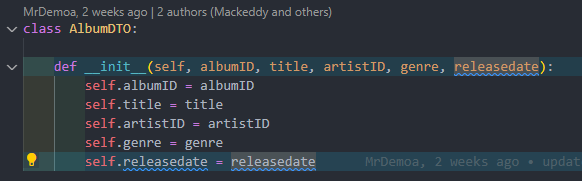
\includegraphics[width=\textwidth]{AlbumDTO.png}
	\end{figure}
\end{flushleft}
\begin{flushleft}
	\begin{figure}[h]
		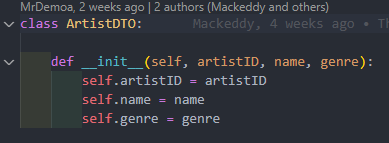
\includegraphics[width=\textwidth]{ArtistDTO.png}
		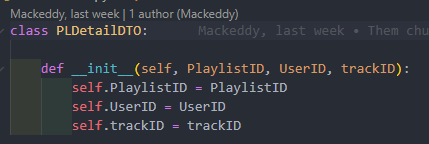
\includegraphics[width=\textwidth]{PlayListDetailDTO.png}
		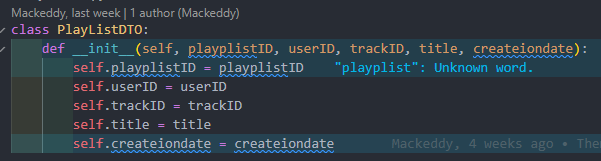
\includegraphics[width=\textwidth]{PlayListDTO.png}
		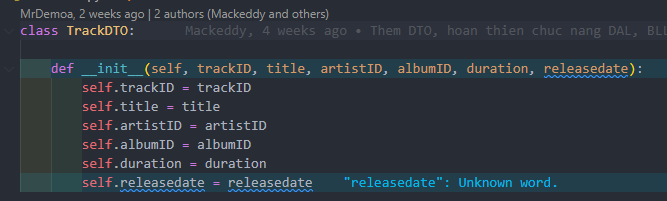
\includegraphics[width=\textwidth]{TrackDTO.png}
	\end{figure}
\end{flushleft}
\clearpage

\newpage
\begin{flushleft}
	\begin{figure}[h]
		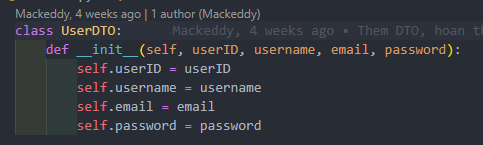
\includegraphics[width=\textwidth]{UserDTO.png}
		\caption{Các class DTO}
	\end{figure}
	-Sau khi chúng ta đã tạo các class DTO, chúng ta sẽ tiến hành tạo các class ở tầng DAL (Data Access Layer) để thực hiện các thao tác truy vấn, cập nhật dữ liệu từ cơ sở dữ liệu:
\end{flushleft}
\begin{figure}[h]
	\centering
	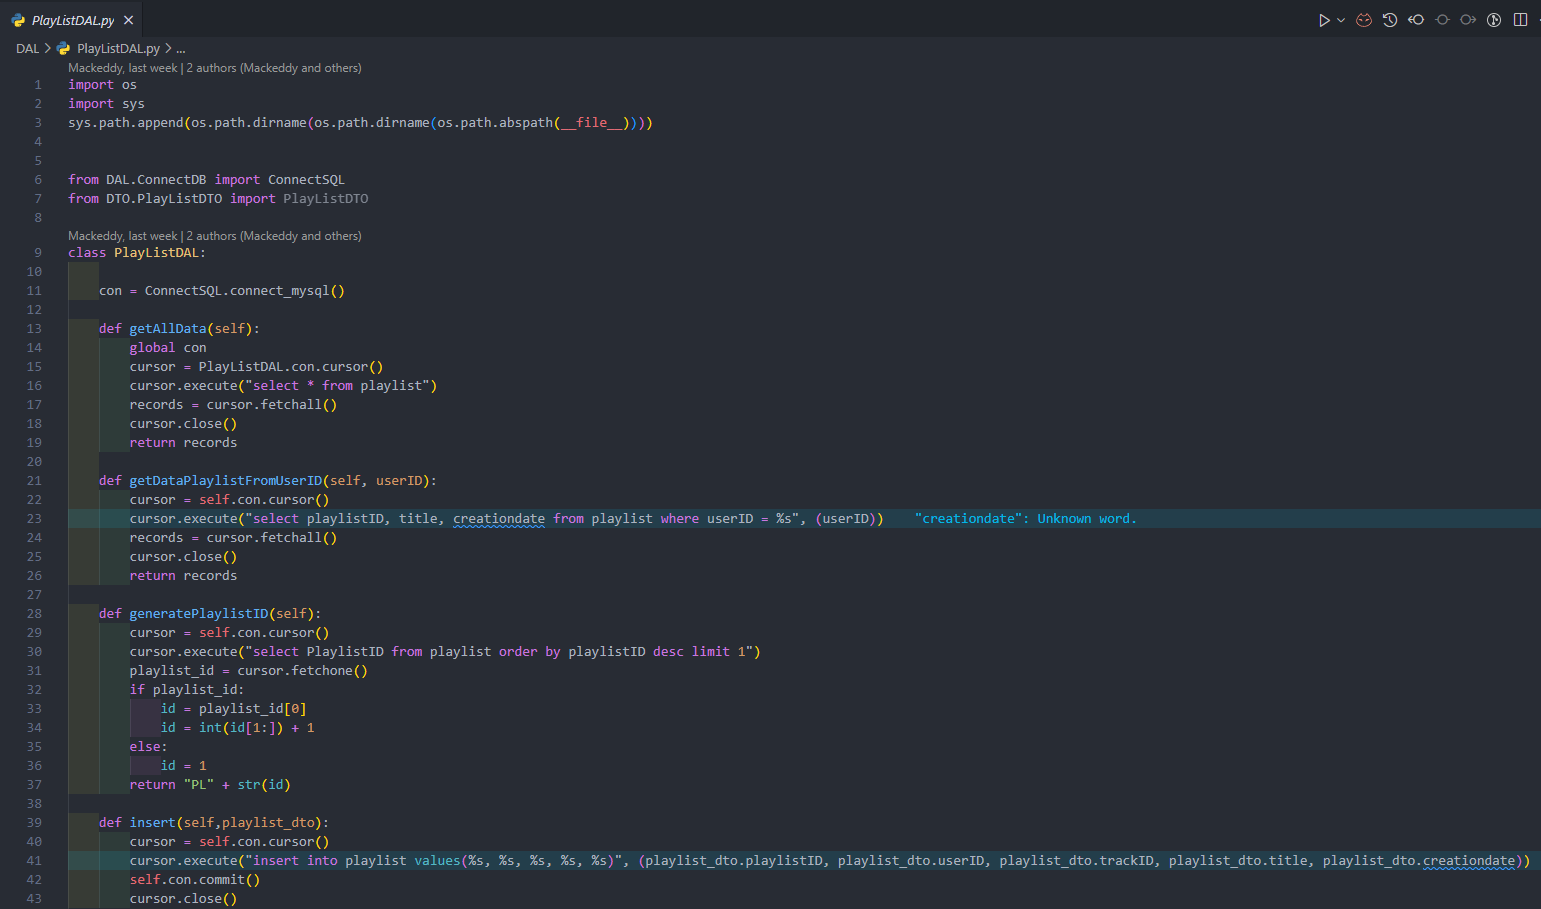
\includegraphics[width=\textwidth]{PlaylistDAL-1.png}
\end{figure}
\begin{figure}
	\includegraphics[width=\textwidth]{PlaylistDAL-2.png}
	\caption{Code cho class PlaylistDAL gồm các phương thức CRUD (Create, Read, Update, Delete)}
\end{figure}

\begin{flushleft}
	-Giải thích:
	\begin{itemize}
		\item Phương thức \textbf{getAllData(self)} trả về danh sách tất cả các playlist trong cơ sở dữ liệu.
		      \begin{flushleft}
			      +Chi tiết hơn:

			      -Đầu tiên, ta sẽ thiết lập kết nối đến cơ sở dữ liệu thông qua class ConnectDB.

			      -Sau đó, ta sẽ tạo 1 cursor để thực hiện các thao tác truy vấn dữ liệu.

			      -Cuối cùng, ta sẽ thực hiện truy vấn dữ liệu và trả về kết quả lưu về records
		      \end{flushleft}
		\item Phương thức \textbf{getDataPlayListFromUserId(self, userID)} trả về thông tin chi tiết của một playlist dựa vào id.
		      \begin{flushleft}
			      +Chi tiết hơn:

			      -Đầu tiên, ta sẽ thiết lập kết nối đến cơ sở dữ liệu thông qua class ConnectDB.

			      -Sau đó, ta sẽ tạo 1 cursor để thực hiện các thao tác truy vấn dữ liệu.

			      -Cuối cùng, ta sẽ thực hiện truy vấn dữ liệu và trả về kết quả lưu về records (trong trường hợp này, ta sẽ truy vấn dữ liệu dựa vào id của user).
		      \end{flushleft}
		\item Phương thức \textbf{generatePlayListID(self)} tạo một ID duy nhất cho playlist mới.
		      \begin{flushleft}
			      +Chi tiết hơn:

			      -Đầu tiên, ta sẽ thiết lập kết nối đến cơ sở dữ liệu thông qua class ConnectDB.

			      -Sau đó, ta sẽ tạo 1 cursor để thực hiện các thao tác truy vấn dữ liệu.

			      -Lấy ra kết quả đầu tiên của query, kiểm tra xem nếu nó tồn tại thì
			      lấy ID đó, loại bỏ ký tự đầu tiên (giả sử là 'PL'), chuyển phần còn lại thành số và cộng thêm một.
			      Điều này đảm bảo rằng mỗi playlist có một ID duy nhất.

			      Nếu không nhận được ID trả về, điều đó có nghĩa là chưa có playlist nào trong cơ sở dữ liệu.
			      Vì vậy, nó đơn giản là đặt ID cho playlist mới là 1.

			      Cuối cùng, nó thêm 'PL' vào đầu ID (để chỉ ra rằng đó là Playlist ID) và trả về nó.
			      Đây sẽ là ID duy nhất cho playlist mới.
		      \end{flushleft}
		\item Phương thức \textbf{insert(self, playlist\_dto)} thêm một playlist mới vào cơ sở dữ liệu.
		      \begin{flushleft}
			      +Chi tiết hơn:

			      -Đầu tiên, ta sẽ thiết lập kết nối đến cơ sở dữ liệu thông qua class ConnectDB.

			      -Sau đó, ta sẽ tạo 1 cursor để thực hiện các thao tác truy vấn dữ liệu.

			      -Sau khi chuẩn bị xong câu lệnh, nó được thực thi bằng cách sử dụng con trỏ (Cursor). Điều này thêm playlist mới vào cơ sở dữ liệu.

			      -Tuy nhiên, chỉ thực thi câu lệnh không đủ. Các thay đổi cần được lưu lại. Đó là lý do tại sao self.con.commit() được sử dụng - nó lưu lại bất kỳ thay đổi nào được thực hiện kể từ lần cuối cùng thay đổi được lưu lại.

			      -Cuối cùng, con trỏ được đóng. Điều này được thực hiện khi chúng ta đã hoàn thành với nó, để giải phóng tài nguyên.
		      \end{flushleft}
		\item Phương thức \textbf{deletePlayList(playlistID)} xóa một playlist dựa vào id.
		      \begin{flushleft}
			      +Chi tiết hơn:

			      -Đầu tiên, ta thiết lập kết nối và tạo con trỏ (Cursor).

			      -Sau đó, ta thực thi câu lệnh DELETE để xóa playlist dựa vào id và đếm số lượng dòng bị ảnh hưởng.

			      -Nếu số lượng dòng bị ảnh hưởng lớn hơn 0, điều đó có nghĩa là playlist đã được xóa thành công.

			      -Cuối cùng, ta lưu lại các thay đổi và đóng con trỏ.
		      \end{flushleft}
		\item Phương thức \textbf{updatePlayList(playlist\_dto)} cập nhật thông tin của một playlist.
		      \begin{flushleft}
			      +Cách thức hoạt động tương tự như phương thức insert, nhưng thay vì thêm mới, nó sẽ cập nhật thông tin của playlist đã tồn tại.
		      \end{flushleft}
	\end{itemize}
\end{flushleft}

\clearpage
\newpage
\begin{figure}[h]
	\centering
	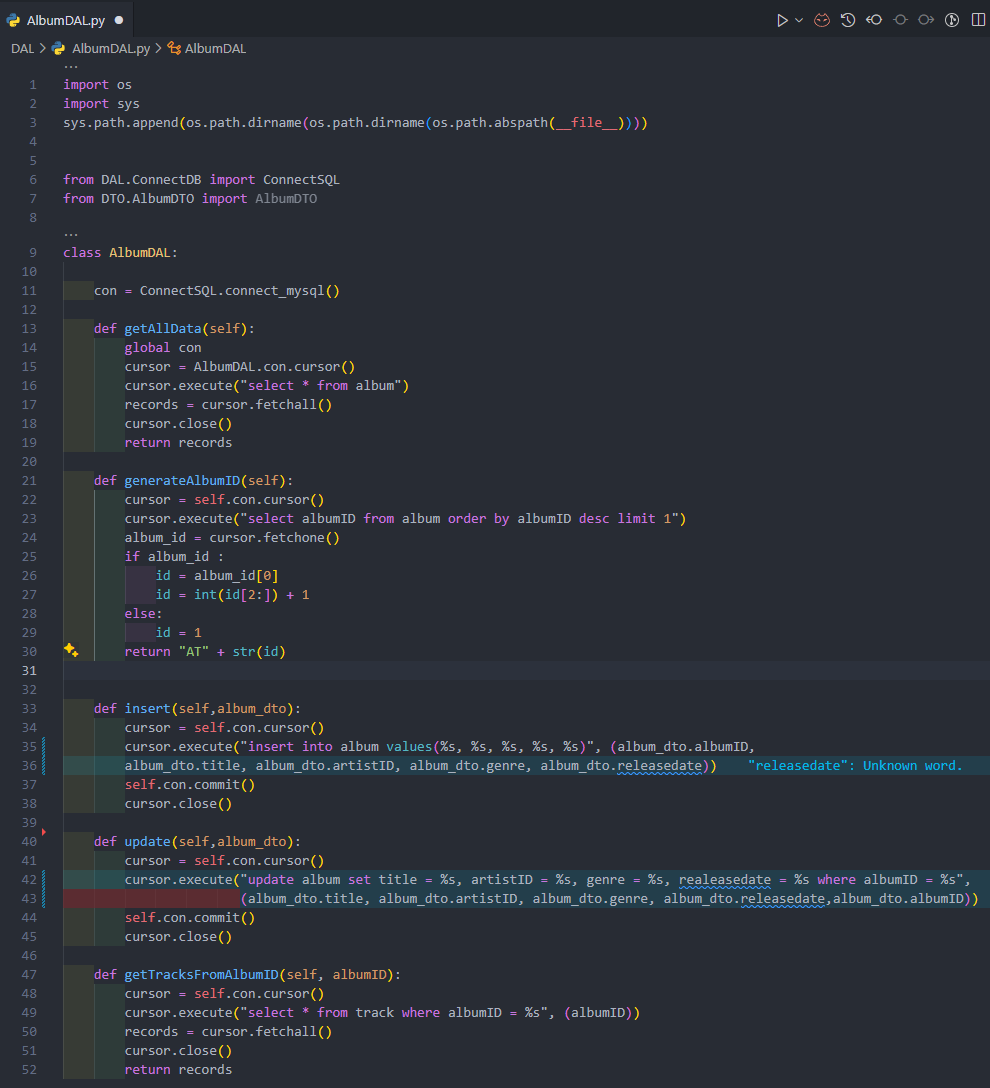
\includegraphics[width=0.9\textwidth]{albumDAL.png}
	\caption{Code cho class AlbumDAL gồm các phương thức đọc, thêm, sửa}
\end{figure}

\begin{flushleft}
	-Giải thích:
	\begin{itemize}
		\item Phương thức \textbf{getAllData(self)} trả về danh sách tất cả các album trong cơ sở dữ liệu.
		      \begin{flushleft}
			      + Tương tự như PlayListDAL chỉ khác là trả về danh sách album.
		      \end{flushleft}
		\item Phương thức \textbf{generateAlbumID(self, albumID)} tạo một ID duy nhất cho album mới.
		      \begin{flushleft}
			      +Chi tiết hơn:

			      -Đầu tiên, chúng ta thiết lập kết nối với cơ sở dữ liệu.

			      -Sau đó, chúng ta yêu cầu cơ sở dữ liệu trả về ID của album được thêm gần đây nhất. Chúng ta làm điều này bằng cách chạy một lệnh yêu cầu "cho tôi albumID từ bảng album, nhưng hãy đảm bảo rằng bạn đưa cho tôi cái cuối cùng bạn có".

			      -Bây giờ, có hai khả năng: hoặc chúng ta nhận được một ID trả về, hoặc không. Nếu chúng ta nhận được một ID, điều đó có nghĩa là đã có một số album trong cơ sở dữ liệu. Vì vậy, chúng ta lấy ID đó, loại bỏ hai ký tự đầu tiên (giả sử là 'AT'), chuyển phần còn lại thành một số và cộng thêm một vào nó. Điều này đảm bảo rằng mỗi album có một ID duy nhất.

			      -Nếu chúng ta không nhận được ID trả về, điều đó có nghĩa là chưa có album nào trong cơ sở dữ liệu. Vì vậy, chúng ta đơn giản là đặt ID cho album mới là 1.

			      -Cuối cùng, chúng ta thêm 'AT' vào đầu ID (để chỉ ra rằng đó là Album ID), và trả về nó. Đây sẽ là ID duy nhất cho album mới.
		      \end{flushleft}
		\item Phương thức \textbf{insert(self, album\_dto)} tạo một album mới trong cơ sở dữ liệu.
		      \begin{flushleft}
			      +Tương tự như hàm insert của PlayListDAL chỉ khác là thêm mới album.
		      \end{flushleft}
		\item Phương thức \textbf{update(album\_dto)} sửa thông tin của một album.
		      \begin{flushleft}
			      +Tương tự như hàm update của PlayListDAL chỉ khác là sửa album.
		      \end{flushleft}
		\item Phương thức \textbf{getTracksFromAlbumID(self, albumID)} lấy ra danh sách các bài hát theo albumID.
		      \begin{flushleft}
			      +Tương tự như hàm getDataPlayListFromUserId của PlayListDAL chỉ khác là lấy ra danh sách bài hát theo albumID.
		      \end{flushleft}
	\end{itemize}
\end{flushleft}
\clearpage

\newpage
\begin{figure}[h]
	\centering
	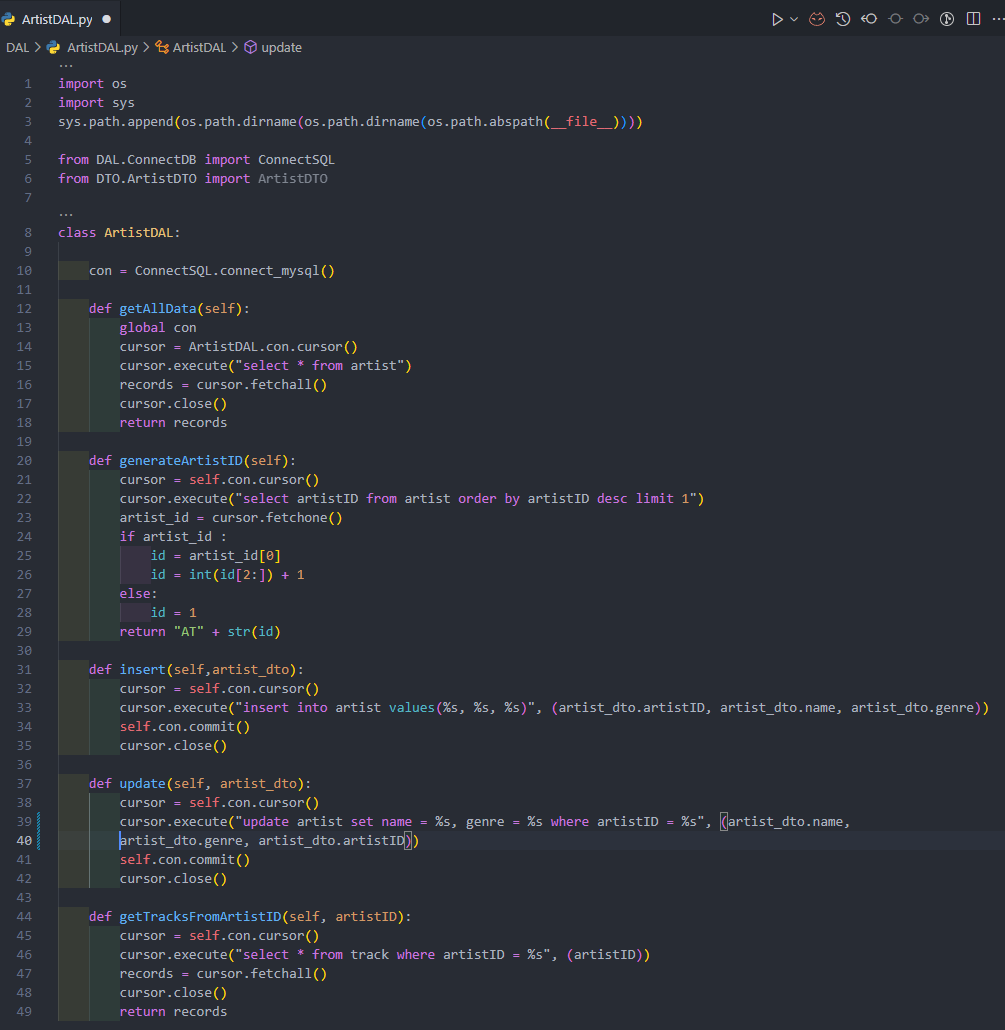
\includegraphics[width=\textwidth]{artistDAL.png}
	\caption{Code cho class ArtistDAL gồm các phương thức đọc, thêm, sửa}
\end{figure}
\begin{flushleft}
	-Giải thích:
	\begin{itemize}
		\item Phương thức \textbf{getAllData(self)} trả về danh sách tất cả các nghệ sĩ trong cơ sở dữ liệu.

		\item Phương thức \textbf{generateArtistID(self)} tạo một ID duy nhất cho nghệ sĩ mới.

		\item Phương thức \textbf{insert(self, artist\_dto)} thêm một nghệ sĩ mới vào cơ sở dữ liệu.

		\item Phương thức \textbf{update(artist\_dto)} sửa thông tin của một nghệ sĩ.

		\item Phương thức \textbf{getTracksFromArtistID(self, artistID)} lấy ra danh sách các bài hát theo artistID.

	\end{itemize}
\end{flushleft}
\clearpage
\newpage
\begin{figure}[h]
	\centering
	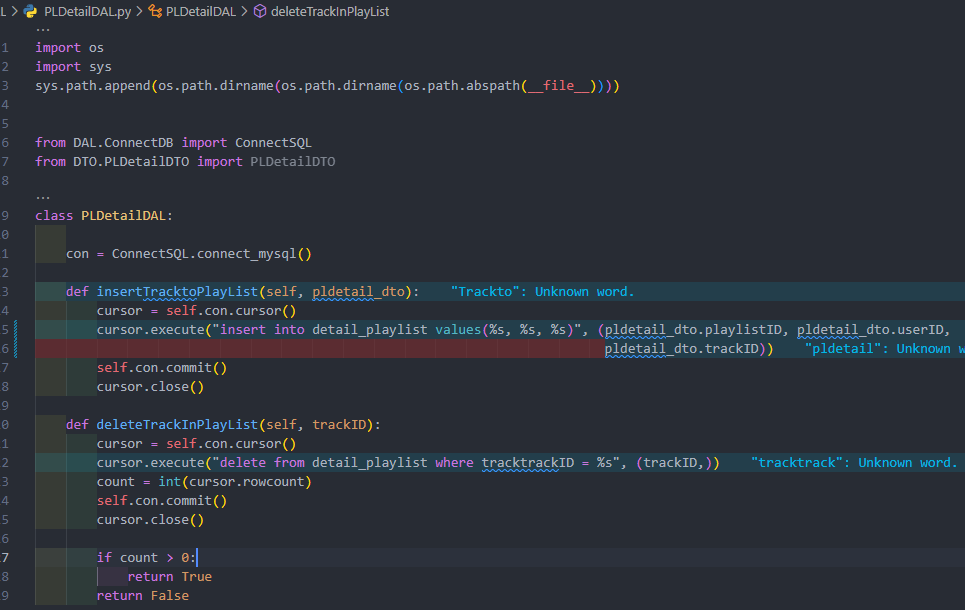
\includegraphics[width=\textwidth]{PlayListDetail.png}
	\caption{Code cho class PLDetailDAL gồm 2 phương thức thêm và xóa}
\end{figure}
\begin{flushleft}
	-Giải thích:
	\begin{itemize}
		\item Phương thức \textbf{insertTracktoPlayList(self, pldetail\_dto)} thêm một bài hát vào playlist.

		\item Phương thức \textbf{deleteTrackInPlayList(playlistID, trackID)} xóa một bài hát khỏi playlist theo trackID.

	\end{itemize}
\end{flushleft}

\clearpage
\newpage
\begin{figure}[h]
	\centering
	\includegraphics[width=\textwidth]{trackDAl.png}
	\caption{Code cho class TrackDAL gồm các phương thức CRUD (Create, Read, Update, Delete)}
\end{figure}
\clearpage
\newpage
\begin{flushleft}
	-Giải thích:
	\begin{itemize}
		\item Phương thức \textbf{getAllData(self)} trả về danh sách tất cả các bài hát trong cơ sở dữ liệu.

		\item Phương thức \textbf{generateTrackID(self)} tạo một ID duy nhất cho bài hát mới.

		\item Phương thức \textbf{insert(self, track\_dto)} thêm một bài hát mới vào cơ sở dữ liệu.

		\item Phương thức \textbf{update(track\_dto)} sửa thông tin của một bài hát.

		\item Phương thức \textbf{deleteTrack(trackID)} xóa một bài hát dựa vào id.

	\end{itemize}
\end{flushleft}
\clearpage

\newpage
\begin{figure}[h]
	\centering
	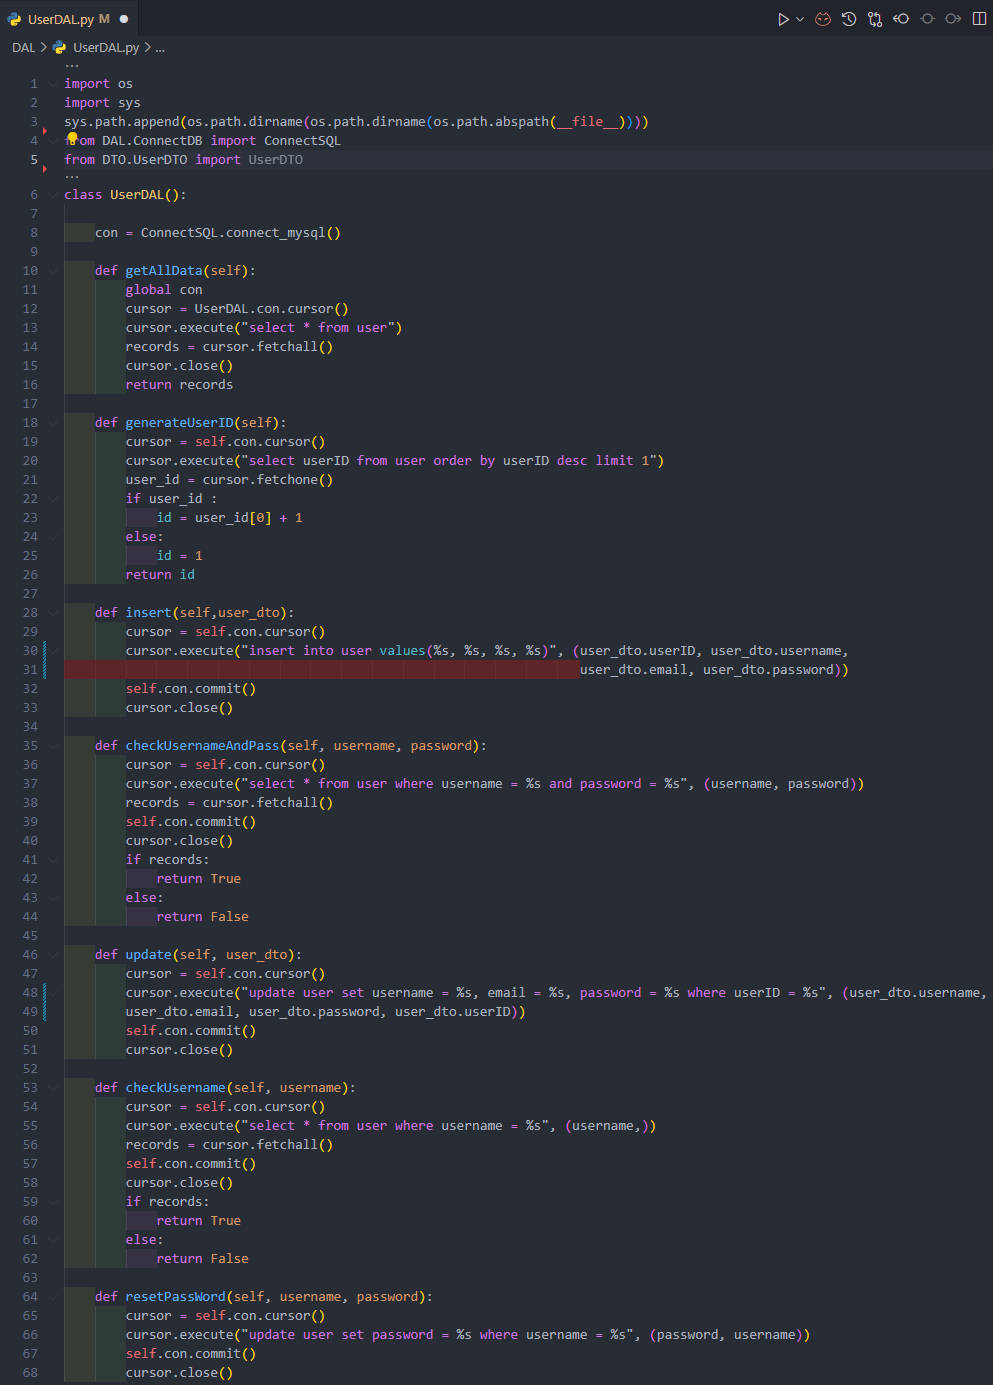
\includegraphics[width=\textwidth]{userDAL.png}
	\caption{Code cho class UserDAL gồm các phương thức CRUD (Create, Read, Update, Delete)}
\end{figure}
\clearpage
\newpage
\begin{flushleft}
	-Giải thích:
	\begin{itemize}
		\item Phương thức \textbf{getAllData(self)} trả về danh sách tất cả các user trong cơ sở dữ liệu.

		\item Phương thức \textbf{generateUserID(self)} tạo một ID duy nhất cho user mới.

		\item Phương thức \textbf{checkUsernameAndPass(self, user\_dto)} kiểm tra username và password của user.

		\item Phương thức \textbf{insert(self, user\_dto)} thêm một user mới vào cơ sở dữ liệu.

		\item Phương thức \textbf{update(self, user\_dto)} sửa thông tin của một user.

		\item Phương thức \textbf{checkUsername(self, userID)} kiểm tra username của user.

		\item Phương thức \textbf{resetPassword(self, username, password)} reset password của user.

	\end{itemize}
	-Sau khi hoàn thành các class ở tầng DAL, chúng ta sẽ tiến hành tạo các class ở tầng BLL (Business Logic Layer) để thực hiện các thao tác xử lý logic cho ứng dụng.
	\begin{figure}[h]
		\centering
		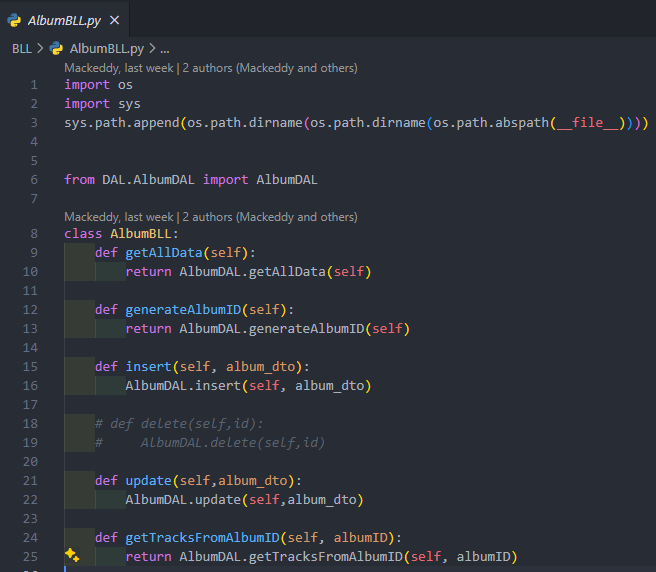
\includegraphics[width=0.9\textwidth]{AlbumBLL.png}
		\caption{Code cho class AlbumBLL gồm các phương thức xử lý logic}
	\end{figure}

\end{flushleft}
\clearpage
\newpage
\begin{figure}[h]
	\centering
	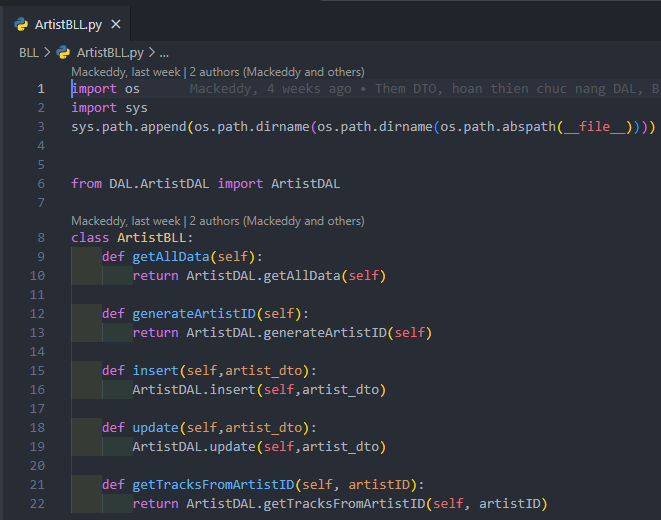
\includegraphics[width=0.8\textwidth]{artistBLL.png}
	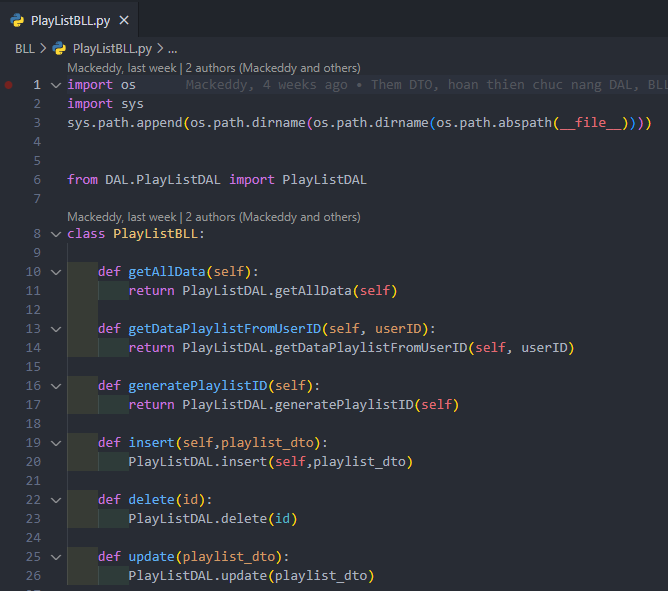
\includegraphics[width=0.8\textwidth]{PlayListBLL.png}
	\caption{Code cho class ArtistBLL, PlayListBLL gồm các phương thức xử lý logic}
\end{figure}

\clearpage
\newpage
\begin{figure}[h]
	\centering
	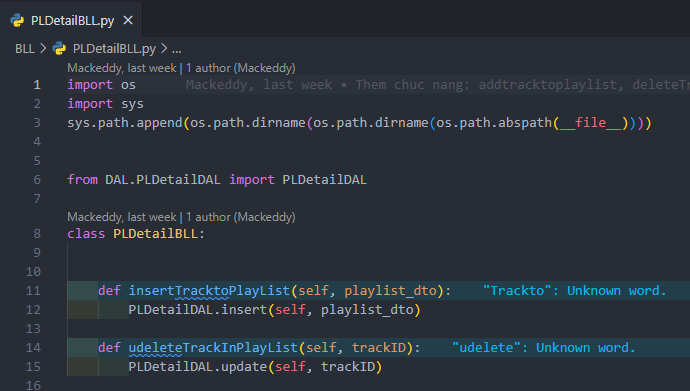
\includegraphics[width=0.8\textwidth]{PLDetailBLL.png}
	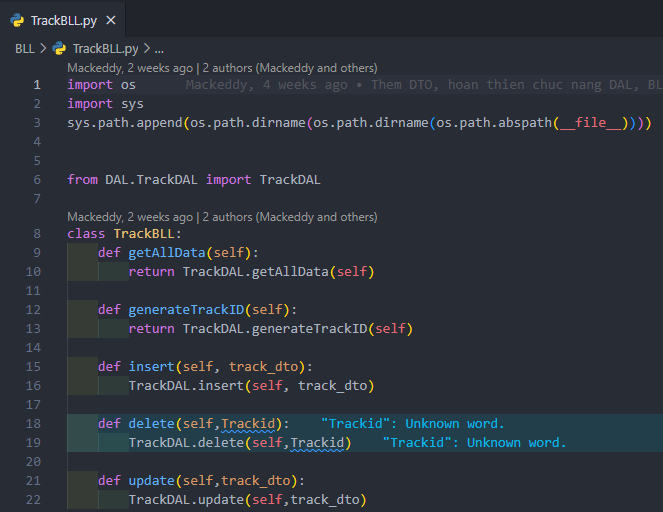
\includegraphics[width=0.8\textwidth]{TrackBLL.png}
	\caption{Code cho class PLDetailBLL, TrackBLL gồm các phương thức xử lý logic}
\end{figure}
\clearpage
\newpage
\begin{figure}[h]
	\centering
	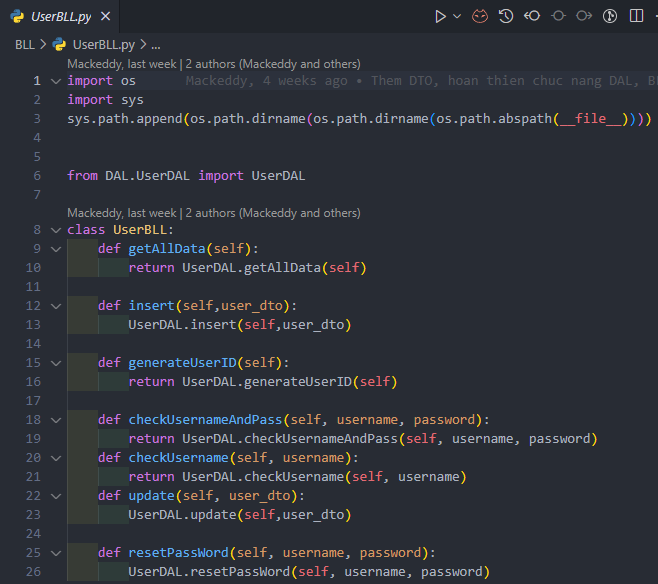
\includegraphics[width=0.8\textwidth]{UserBLL.png}
	\caption{Code cho class UserBLL gồm các phương thức xử lý logic}
\end{figure}
\begin{flushleft}
	-Sau khi hoàn thành việc thiết lập các phương thức xử lý tại các tầng BLL và DAL,
	chúng ta sẽ tiếp tục tạo các lớp (class) tại tầng GUI (Graphical User Interface). Mục đích của việc này là để thực hiện các thao tác giao diện cho ứng dụng.

	-Đồng thời, chúng ta sẽ sử dụng thư viện Tkinter để tạo giao diện cho ứng dụng.
	Thư viện Pygame.mixer sẽ được sử dụng để phát nhạc trong ứng dụng.

	-Ngoài ra, chúng ta cũng sẽ sử dụng thư viện socket để tạo kết nối giữa client và server.
	Điều này giúp cho việc truyền dữ liệu giữa client và server trở nên dễ dàng hơn.
\end{flushleft}
\newpage
\begin{thebibliography}{80}

	\bibitem{CVX}
	CVX Introduction
	``\textbf{link: http://cvxr.com/cvx/doc/intro.html/}'',
	\textit{What is CVX}, lần truy cập cuối: 15/04/2017.

\end{thebibliography}
\end{document}